%====================================================
% Informe Final - Proyecto Central VoIP
% Asignatura: Comunicación de Datos
% Autores: Adrián Campos (CI 30.513.493)
%          Aaron Contreras (CI 31.871.275)
%====================================================
\documentclass[12pt,a4paper]{article}

%----------------------------------------------------
% Paquetes fundamentales
%----------------------------------------------------
\usepackage{fontspec}
\usepackage[spanish]{babel}

% Fuente Arial 12pt (se utiliza TeX Gyre Heros, metricamente compatible con Arial)
\setmainfont{TeX Gyre Heros}[BoldFont={TeX Gyre Heros Bold}, ItalicFont={TeX Gyre Heros Italic}]

% Tamaño base 12pt ya definido en documentclass
\fontsize{12pt}{18pt}\selectfont

% Color de texto #121212
\usepackage{xcolor}
\definecolor{textcolor}{HTML}{121212}
\color{textcolor}

% Margenes APA UPEL: 2.54 cm en todos los lados
\usepackage[margin=2.54cm]{geometry}

% Interlineado 1.5
\usepackage{setspace}
\onehalfspacing

% Encabezados y pie de pagina
\usepackage{fancyhdr}
\setlength{\headheight}{14.5pt}
\pagestyle{fancy}
\fancyhf{}
\fancyhead[R]{\thepage}
\fancyhead[L]{\small Implementación y Administración de una Central VoIP}
\renewcommand{\headrulewidth}{0.4pt}

% Secciones y subsecciones
\usepackage{titlesec}
\titleformat{\section}{\normalfont\bfseries\large}{\thesection.}{0.5em}{}
\titleformat{\subsection}{\normalfont\bfseries}{\thesubsection.}{0.5em}{}
\titleformat{\subsubsection}{\normalfont\bfseries\itshape}{\thesubsubsection.}{0.5em}{}

% Tablas y figuras
\usepackage{graphicx}
\usepackage{booktabs}
\usepackage{caption}
\captionsetup{font=small,labelfont=bf}
\usepackage{float}

% Listas
\usepackage{enumitem}
\setlist{nosep,leftmargin=*}

% Código fuente y comandos
\usepackage{listings}
\lstset{
    basicstyle=\ttfamily\small,
    breaklines=true,
    frame=single,
    backgroundcolor=\color{gray!10},
    rulecolor=\color{gray!50},
    showstringspaces=false,
    tabsize=2
}

% Diagramas
\usepackage{tikz}
\usetikzlibrary{shapes.geometric, shapes.symbols, arrows.meta, positioning, fit, backgrounds, calc, babel}

% Hipervinculos
\usepackage{hyperref}
\usepackage{bookmark}
\hypersetup{
    colorlinks=true,
    linkcolor=textcolor,
    urlcolor=textcolor,
    citecolor=textcolor,
    pdftitle={Informe Final - Proyecto Central VoIP},
    pdfauthor={Adrian Campos y Aaron Contreras}
}

% Cajas para capturas de pantalla
\usepackage{fancybox}

% Otros utilitarios
\usepackage{array}
\usepackage{longtable}
\usepackage{multicol}

% Espaciado de parrafos
\setlength{\parskip}{0.5em}
\setlength{\parindent}{1.27cm}

%====================================================
% Inicio del documento
%====================================================
\begin{document}

%----------------------------------------------------
% PORTADA
%----------------------------------------------------
\definecolor{ucvblue}{HTML}{1A3C6D}

\begin{titlepage}
    \centering
    \vspace*{0.5cm}

    % --- Encabezado Institucional ---
    {\large\bfseries Universidad Central de Venezuela}\\[0.2cm]
    {\large Facultad de Ciencias}\\[0.2cm]
    {\large Escuela de Computación}\\[0.2cm]
    {\normalsize Asignatura: Comunicación de Datos}\\[2.5cm]

    % --- Bloque de Título con filete de color ---
    {\color{ucvblue}\rule{\linewidth}{1.8pt}}\\[0.6cm]
    {\huge\bfseries Implementación y Administración\\[0.3cm] de una Central VoIP}\\[0.5cm]
    {\large\itshape Proyecto Final --- Informe Técnico}\\[0.4cm]
    {\color{ucvblue}\rule{\linewidth}{1.8pt}}\\[3cm]

    % --- Datos del Proyecto / Autores ---
    \begin{minipage}{0.85\linewidth}
        \renewcommand{\arraystretch}{1.4}
        \begin{tabular}{@{}lllll@{}}
            \textbf{Autores:} & Adrián Campos    & \hspace{0.5cm} & C.I.: & 30.513.493 \\
                              & Aaron Contreras  & \hspace{0.5cm} & C.I.: & 31.871.275 \\[0.3cm]
            \textbf{Cliente:} & \multicolumn{4}{l}{NovaLink C.A.} \\
            \textbf{Fecha:}   & \multicolumn{4}{l}{Septiembre 2026} \\
        \end{tabular}
    \end{minipage}

    \vfill

    % --- Pie de página ---
    {\normalsize Caracas, Venezuela}
    \vspace*{0.5cm}
\end{titlepage}

%----------------------------------------------------
% INDICE (tamaño reducido para que quepa en una página)
%----------------------------------------------------
\newpage
\thispagestyle{empty}
\begin{center}
    {\Large\bfseries Índice de Contenido}
\end{center}
\vspace{0.3cm}
{
\footnotesize
\renewcommand{\contentsname}{}
\setlength{\parskip}{0pt}
\setlength{\parindent}{0pt}
\tableofcontents
}
\vfill
\thispagestyle{fancy}
\newpage

%----------------------------------------------------
% RESUMEN
%----------------------------------------------------
\section{Resumen}

El presente informe documenta el diseño, implementación, despliegue y validación de una central telefónica basada en VoIP para la organización ficticia NovaLink C.A. La solución utiliza Asterisk 20 compilado manualmente desde su código fuente, desplegado dentro de contenedores Docker sobre Linux Ultramarine 43. Se emplean los protocolos SIP/PJSIP para la señalización, RTP/SDP para el transporte de medios, y se contemplan mecanismos de seguridad mediante autenticación digest, TLS y SRTP.

La central soporta llamadas internas entre extensiones, interconexión con otra central mediante troncal SIP/PJSIP, funciones PBX como retención, transferencia, conferencia, así como un escenario de Hold con configuración de timeout a los 15 minutos. La conectividad entre sedes se realiza mediante ZeroTier, una red virtual definida por software que permite la comunicación punto a punto a través de Internet.

Se incluyen capturas de tráfico realizadas con Asterisk CLI y análisis SIP para la validación del comportamiento de la señalización y los flujos de audio.

\textbf{Palabras clave:} VoIP, Asterisk, SIP, PJSIP, RTP, SDP, TLS, SRTP, Docker, PBX, troncal SIP, ZeroTier.

%----------------------------------------------------
% INTRODUCCION
%----------------------------------------------------
\section{Introducción}

La evolución de las telecomunicaciones ha migrado progresivamente de las redes telefónicas conmutadas tradicionales (PSTN) hacia arquitecturas basadas en IP. La Voz sobre IP (VoIP) permite transportar comunicaciones de voz sobre redes de datos, reduciendo costos, aumentando la flexibilidad e integrando servicios que antes requerían infraestructuras separadas.

NovaLink C.A., organización ficticia con cinco sedes distribuidas en distintas regiones de Venezuela, requiere una solución de telefonía unificada que permita comunicaciones internas entre sus extensiones, salidas hacia redes externas y la interconexión con otras centrales. El presente proyecto responde a esta necesidad mediante el despliegue de una central Asterisk containerizada, con soporte para señalización SIP/PJSIP, transporte RTP/SDP, múltiples codecs de audio, troncales SIP y funciones empresariales de PBX.

El objetivo principal es entregar una solución funcional, documentada y reproducible, capaz de ser trasladada al servidor asignado por CICORE y verificada mediante pruebas de registro, llamadas internas, llamadas por troncal, capturas de tráfico y funciones PBX adicionales.

%----------------------------------------------------
% MARCO TEORICO
%----------------------------------------------------
\section{Marco Teórico}

\subsection{Protocolo SIP (Session Initiation Protocol)}

SIP es el protocolo estándar de facto para la señalización en VoIP, definido por la IETF en la RFC 3261 \cite{rfc3261}. Opera en la capa de aplicación y se encarga de establecer, modificar y terminar sesiones de comunicación entre usuarios. SIP no transporta la voz; su función es negociar parámetros de llamada, localizar usuarios dentro de la red y gestionar el estado de las sesiones mediante métodos como INVITE, ACK, BYE, REGISTER, CANCEL y re-INVITE.

\subsection{Protocolo RTP (Real-Time Transport Protocol)}

Una vez establecida la sesión por SIP, RTP se utiliza para transportar el flujo de audio digitalizado en tiempo real, según lo especificado en la RFC 3550 \cite{rfc3550}. RTP opera sobre UDP para reducir la latencia y la sobrecarga, sacrificando confiabilidad en favor de velocidad, lo cual es esencial en comunicaciones de voz interactivas.

\subsection{SDP (Session Description Protocol)}

SDP, definido en la RFC 4566, es el formato utilizado por SIP para describir los parámetros de las sesiones multimedia. SDP incluye información sobre direcciones IP, puertos RTP, codecs soportados, perfiles de seguridad y atributos de media, como \texttt{a=sendrecv}, \texttt{a=sendonly} o \texttt{a=inactive}.

\subsection{Codecs de Audio}

Los codecs son algoritmos encargados de codificar y comprimir el audio analógico en paquetes de datos digitales. El proyecto utiliza G.711 (ulaw y alaw) como referencia funcional, por su alta calidad y baja latencia, y contempla G.729 como codec alternativo para optimización de ancho de banda \cite{itu_g}.

\subsection{Asterisk PBX}

Asterisk es un framework de código abierto que actúa como motor central de conmutación de llamadas (PBX) \cite{asterisk_book}. Su administración pura requiere comprender su arquitectura interna y manipular directamente archivos de configuración para definir canales de comunicación, reglas de enrutamiento y lógica de llamadas.

\subsection{Troncales SIP y Conexión entre Centrales}

Una troncal SIP o PJSIP permite interconectar dos centrales telefónicas independientes para intercambiar llamadas entre dominios distintos. Mediante autenticación, reglas de identificación y planes de marcado coordinados, dos PBX pueden comportarse como parte de una misma red de comunicaciones.

\subsection{Seguridad en VoIP}

La seguridad en VoIP incluye autenticación de usuarios mediante digest, cifrado de señalización mediante TLS y cifrado del audio mediante SRTP. Estas medidas reducen la exposición de credenciales, protegen el contenido de las llamadas y robustecen el servicio frente a accesos no autorizados.

\subsection{ZeroTier}

ZeroTier es una red virtual definida por software (SDN) que permite crear redes punto a punto cifradas a través de Internet. Cada dispositivo se asigna a una red virtual con un identificador único y recibe una IP dentro de un rango configurado. En este proyecto, ZeroTier se utiliza para conectar las sedes de NovaLink C.A. sin necesidad de VPN tradicional ni configuración de port forwarding.

\subsection{Calidad de Servicio y Métricas}

La calidad de una llamada VoIP depende de factores como latencia, jitter, pérdida de paquetes y estabilidad del audio. Estos indicadores permiten evaluar la experiencia del usuario y diagnosticar problemas de red o configuración.

\subsection{Servicios Básicos de una PBX}

Además de originar y recibir llamadas, una central telefónica ofrece funciones como transferencia, retención, llamada en espera, conferencia, acercando la solución a un escenario de uso empresarial.

\subsection{Plan de Numeración y Enrutamiento}

El plan de numeración define cómo se identifican las extensiones y qué prefijos se utilizan para distinguir sedes, servicios o destinos externos. A partir de este esquema se organiza el enrutamiento de llamadas entrantes y salientes.

%----------------------------------------------------
% REQUERIMIENTOS DEL CLIENTE
%----------------------------------------------------
\section{Requerimientos del Cliente}

NovaLink C.A. establece los siguientes requerimientos para la solución de telefonía unificada:

\begin{enumerate}
    \item Plataforma Linux con central Asterisk compilada manualmente desde código fuente.
    \item Despliegue containerizado mediante Docker, incluyendo configuración y dependencias.
    \item Señalización mediante SIP/PJSIP y transporte de audio mediante RTP/SDP.
    \item Soporte para al menos dos extensiones SIP registradas simultáneamente.
    \item Soporte de múltiples codecs, con G.711 como referencia funcional.
    \item Interconexión con otra central VoIP mediante troncal SIP/PJSIP.
    \item Mecanismos de seguridad: autenticación, TLS y SRTP.
    \item Captura y análisis de tráfico con Wireshark, tcpdump o equivalentes.
    \item Pruebas funcionales con softphones o herramientas SIP equivalentes.
    \item Plan de numeración claro con prefijos para internas, entrantes y salientes.
    \item Escenario de Hold con timeout configurado a los 15 minutos.
    \item Registro de eventos, diagnósticos y anomalías en archivos log.
    \item Funciones PBX adicionales: retención, transferencia y conferencia.
    \item Verificación de calidad de voz mediante indicadores de operación.
    \item Informe final con arquitectura de solución, topología, medio de transmisión y justificación técnica.
\end{enumerate}

%----------------------------------------------------
% ARQUITECTURA DE SOLUCION
%----------------------------------------------------
\section{Arquitectura de Solución}

\subsection{Topología Propuesta}

La Figura \ref{fig:topología} presenta la topología general de la solución. La central principal (\texttt{pbx-asterisk}) se despliega en modo host dentro de un contenedor Docker sobre Linux Ultramarine 43, lo que le permite acceder directamente a las interfaces de red del anfitrión, incluyendo loopback (\texttt{127.0.0.1}), red local (\texttt{192.168.123.0/24}) y red ZeroTier (\texttt{10.119.203.0/24}). Una segunda central (\texttt{pbx-remota}) se despliega en red bridge para simular una sede externa interconectada mediante troncal SIP/PJSIP.

La conectividad entre sedes se logra mediante ZeroTier, que asigna IPs dentro del rango \texttt{10.119.203.0/24} a cada dispositivo participante. La máquina del servidor (Adrián) tiene la IP \texttt{10.119.203.172} y la máquina del compañero (Aaron) tiene la IP \texttt{10.119.203.48}.

\begin{figure}[H]
\centering
\begin{tikzpicture}[
    node distance=1.2cm,
    box/.style={rectangle, draw, rounded corners, minimum width=3cm, minimum height=0.8cm, align=center, fill=gray!10},
    smallbox/.style={rectangle, draw, rounded corners, minimum width=2.2cm, minimum height=0.7cm, align=center, fill=gray!5},
    arrow/.style={-{Stealth[scale=0.8]}, thick},
    label/.style={font=\small\itshape}
]

% Nube ZeroTier
\node[rectangle, draw, rounded corners, minimum width=4cm, minimum height=1.5cm, align=center, fill=blue!10] (internet) {ZeroTier /\\10.119.203.0/24};

% Host Docker
\node[rectangle, draw, dashed, minimum width=12cm, minimum height=6.5cm, below=of internet, fill=blue!3] (host) {};
\node[label, anchor=north west] at (host.north west) {\scriptsize Docker Host (Ultramarine Linux 43)};

% PBX Principal
\node[box, below left=1.5cm and 0.5cm of internet] (pbx) {\textbf{pbx-asterisk}\\ Asterisk 20.21.0\\ IP: 10.119.203.172};

% PBX Remota
\node[box, below right=1.5cm and 0.5cm of internet] (remota) {\textbf{pbx-remota}\\ Asterisk 20.21.0\\ Bridge: 172.18.0.50};

% Extensiones
\node[smallbox, below left=1.5cm and 0.3cm of pbx] (ext1001) {1001 - Adrian};
\node[smallbox, below=of ext1001] (ext1002) {1002 - Aaron};

% Extensión remota
\node[smallbox, below=of remota] (ext2001) {2001 - Remota};

% Herramientas de prueba
\node[smallbox, below=2.5cm of pbx] (wireshark) {Linphone 6.2.3};

% Conexiones
\draw[arrow] (internet) -- node[right, font=\scriptsize] {Troncal SIP} (pbx);
\draw[arrow, <->] (pbx) -- node[above, font=\scriptsize] {Troncal SIP} (remota);
\draw[arrow, <->] (pbx) -- (ext1001);
\draw[arrow, <->] (pbx) -- (ext1002);
\draw[arrow, <->] (remota) -- (ext2001);
\draw[arrow, <->] (pbx) -- (wireshark);

\end{tikzpicture}
\caption{Topología general de la solución VoIP}
\label{fig:topología}
\end{figure}

\subsection{Medio de Transmisión Seleccionado}

La Tabla \ref{tab:medio} resume el medio de transmisión seleccionado y su justificación.

\begin{table}[H]
\centering
\caption{Medio de transmisión y justificación}
\label{tab:medio}
\begin{tabular}{@{}p{3.5cm}p{4cm}p{6cm}@{}}
\toprule
\textbf{Aspecto} & \textbf{Selección} & \textbf{Justificación} \\
\midrule
Señalización & SIP sobre UDP/TCP/TLS & Estándar IETF (RFC 3261), ampliamente soportado y escalable. \\
Transporte de medios & RTP sobre UDP & Baja latencia, adecuado para voz en tiempo real (RFC 3550). \\
Infraestructura & Docker sobre Linux & Portabilidad, aislamiento y fácil despliegue. \\
Red interna & Docker bridge / host & Comunicación entre contenedores y acceso directo a interfaces físicas. \\
Red externa & ZeroTier SDN & Conexión punto a punto cifrada entre sedes sin VPN tradicional. \\
Codecs & G.711 (ulaw/alaw), G.729 & G.711 como referencia funcional; G.729 para optimización de ancho de banda. \\
\bottomrule
\end{tabular}
\end{table}

Se elige UDP para SIP y RTP porque la voz en tiempo real prioriza la baja latencia sobre la confiabilidad de entrega. TCP introduce retransmisiones que degradan la experiencia de llamada. TLS se configura opcionalmente para cifrado de señalización y SRTP para cifrado de audio. ZeroTier se utiliza para la conectividad entre sedes, proporcionando una red virtual cifrada con IPs estáticas.

%----------------------------------------------------
% INSTALACION Y CONFIGURACION
%----------------------------------------------------
\section{Instalación, Compilación y Despliegue}

\subsection{Requisitos del Sistema}

\begin{table}[H]
\centering
\caption{Requisitos del sistema}
\label{tab:requisitos}
\begin{tabular}{@{}lcc@{}}
\toprule
\textbf{Componente} & \textbf{Mínimo} & \textbf{Recomendado} \\
\midrule
Sistema operativo & Linux Fedora 40+ & Ultramarine Linux 43 \\
Memoria RAM & 4 GB & 8 GB \\
Disco & 10 GB libres & 20 GB \\
CPU & 2 núcleos & 4 núcleos \\
Docker & 20.10+ & 29.x \\
\bottomrule
\end{tabular}
\end{table}

\subsection{Estructura del Proyecto}

El proyecto se organiza en el directorio \texttt{/home/andriby/central-voip/} con la siguiente estructura:

\begin{lstlisting}
central-voip/
|-- Dockerfile                  # Compilacion de Asterisk desde fuente
|-- docker-compose.yml          # Orquestacion de servicios
|-- conf/
|   |-- pjsip.conf             # Endpoints, autenticacion, troncales, transportes
|   |-- extensions.conf        # Plan de marcado (dialplan)
|   |-- features.conf          # Transferencia, retencion
|   |-- res_parking.conf       # Configuracion de parking (Hold)
|   |-- confbridge.conf        # Conferencias
|   |-- rtp.conf               # Rango de puertos RTP
|   |-- remota/                # Configuracion de PBX remota
|-- certs/
|   |-- asterisk.crt           # Certificado TLS autofirmado
|   |-- asterisk.key           # Clave privada TLS
|-- captures/                   # Capturas de trafico
|-- logs/                       # Logs de Asterisk
\end{lstlisting}

\subsection{Compilación de Asterisk}

El archivo \texttt{Dockerfile} define la compilación manual de Asterisk 20.21.0 desde su código fuente sobre Debian 12 slim. El proceso incluye la instalación de dependencias de compilación, descarga del código fuente, ejecución de \texttt{configure}, selección de módulos mediante \texttt{menuselect}, compilación paralela e instalación.

Se compila con soporte para SRTP incluyendo la dependencia \texttt{libsrtp2-dev} y el módulo \texttt{res\_srtp.so}, habilitado mediante \texttt{--enable res\_srtp} en el comando \texttt{./configure}.

\subsection{Generación de Certificados TLS}

Se genera un certificado autofirmado con validez de un año, incluyendo Subject Alternative Name (SAN) con las direcciones IP utilizadas:

\begin{lstlisting}
openssl req -x509 -newkey rsa:2048 \
  -keyout certs/asterisk.key \
  -out certs/asterisk.crt \
  -days 365 -nodes \
  -subj "/C=VE/ST=Caracas/L=Caracas/O=NovaLink/OU=VoIP/CN=asterisk.novalink.local" \
  -addext "subjectAltName=DNS:asterisk.novalink.local,IP:127.0.0.1,IP:10.119.203.172,IP:192.168.123.12"
\end{lstlisting}

\subsection{Despliegue con Docker Compose}

El despliegue se realiza con el siguiente comando:

\begin{lstlisting}
cd ~/central-voip
docker compose up -d
\end{lstlisting}

El servicio \texttt{pbx-asterisk} utiliza \texttt{network\_mode: host} para acceder directamente a las interfaces de red del anfitrión, con \texttt{extra\_hosts} configurado para resolver el hostname \texttt{ultramarine} a \texttt{127.0.0.1}. El servicio \texttt{pbx-remota} utiliza red bridge con IP estática \texttt{172.18.0.50} y puertos mapeados para acceso externo.

\subsection{Configuración de ZeroTier}

ZeroTier se configura en ambas máquinas participantes. Cada dispositivo se une a la red virtual mediante su identificador de red (\texttt{network id}) y recibe una IP estática dentro del rango \texttt{10.119.203.0/24}:

\begin{table}[H]
\centering
\caption{Asignación de IPs ZeroTier}
\label{tab:zerotier}
\begin{tabular}{@{}llll@{}}
\toprule
\textbf{Dispositivo} & \textbf{Device ID} & \textbf{IP ZeroTier} & \textbf{Rol} \\
\midrule
Adrián (Servidor) & c3d16b7921 & 10.119.203.172 & pbx-asterisk \\
Aaron (Compañero) & 9f9e93aa14 & 10.119.203.48 & pbx-remota / Softphone \\
\bottomrule
\end{tabular}
\end{table}

%----------------------------------------------------
% PLAN DE NUMERACION
%----------------------------------------------------
\section{Plan de Numeración}

La Tabla \ref{tab:numeración} resume el plan de numeración implementado.

\begin{table}[H]
\centering
\caption{Plan de numeración}
\label{tab:numeración}
\begin{tabular}{@{}p{4cm}p{5cm}p{4.5cm}@{}}
\toprule
\textbf{Prefijo / Extensión} & \textbf{Destino} & \textbf{Ejemplo} \\
\midrule
1001, 1002 & Extensiones internas & 1001 $\rightarrow$ Adrian \\
9 + número & Llamada saliente por troncal & 91234567 \\
92 + extensión remota & PBX remota (2XXX) & 92001 \\
00 + número & Llamada internacional por troncal & 005812345 \\
700 & Estacionar llamada (Park) & Durante llamada: \#72 \\
8600 & Sala de conferencia & ConfBridge \\
\bottomrule
\end{tabular}
\end{table}

%----------------------------------------------------
% CONFIGURACION IMPLEMENTADA
%----------------------------------------------------
\section{Configuración Implementada}

\subsection{Credenciales de Acceso}

\begin{table}[H]
\centering
\caption{Credenciales de extensiones y troncal}
\label{tab:credenciales}
\begin{tabular}{@{}lcccp{3cm}@{}}
\toprule
\textbf{Extensión} & \textbf{Nombre} & \textbf{Usuario} & \textbf{Contraseña} & \textbf{Rol} \\
\midrule
1001 & Adrián Campos & 1001 & nova1001 & Extensión interna \\
1002 & Aaron Contreras & 1002 & nova1002 & Extensión interna \\
2001 & Usuario Remoto & 2001 & nova2001 & Extensión remota \\
\bottomrule
\end{tabular}
\end{table}

\subsection{Configuración PJSIP}

Se configuran tres transportes: UDP (5060), TCP (5060) y TLS (5061). Los endpoints 1001 y 1002 incluyen autenticación digest, configuración NAT para ZeroTier (\texttt{rtp\_symmetric=yes}, \texttt{rewrite\_contact=yes}, \texttt{force\_rport=yes}), codecs y timeouts de RTP. La troncal remota se define sin registro, utilizando identificación por IP.

Parámetros clave de los endpoints:

\begin{itemize}
    \item \texttt{media\_encryption=sdes}: Habilita SRTP para cifrado de audio.
    \item \texttt{suppress\_moh\_on\_sendonly=true}: Suprime música en espera cuando el canal recibe \texttt{a=sendonly}.
    \item \texttt{rtp\_timeout\_hold=900}: Timeout de 15 minutos para llamadas en hold.
    \item \texttt{direct\_media=no}: Asterisk actúa como proxy de medios (necesario para NAT/ZeroTier).
    \item \texttt{external\_media\_address=10.119.203.172}: Dirección IP externa para RTP.
\end{itemize}

\subsection{Configuración del Dialplan}

El dialplan organiza las llamadas en contextos:
\begin{itemize}
    \item \texttt{internas}: llamadas entre extensiones 1001 y 1002, funciones PBX (conferencia 8600).
    \item \texttt{outgoing}: llamadas salientes por troncal con prefijos 9 (local) y 00 (internacional). El patrón \texttt{\_92XXX} enruta llamadas a la PBX remota.
    \item \texttt{from-trunk}: llamadas entrantes desde la PBX remota. El patrón \texttt{\_1XXX} enruta a extensiones internas.
\end{itemize}

\subsection{Configuración de Seguridad}

\begin{itemize}
    \item \textbf{Autenticación digest}: Todas las extensiones requieren usuario y contraseña.
    \item \textbf{TLS}: Transporte en puerto 5061 con certificado autofirmado que incluye SAN para DNS e IP.
    \item \textbf{SRTP}: Módulo \texttt{res\_srtp.so} compilado y ejecutándose, con \texttt{media\_encryption=sdes} en los endpoints.
\end{itemize}

%----------------------------------------------------
% PRUEBAS Y RESULTADOS
%----------------------------------------------------
\section{Pruebas y Resultados}

\subsection{Registro de Extensiones}

Ambas extensiones se registran correctamente en la central. La Figura \ref{fig:registro} muestra el estado de los endpoints.

\begin{figure}[H]
\centering
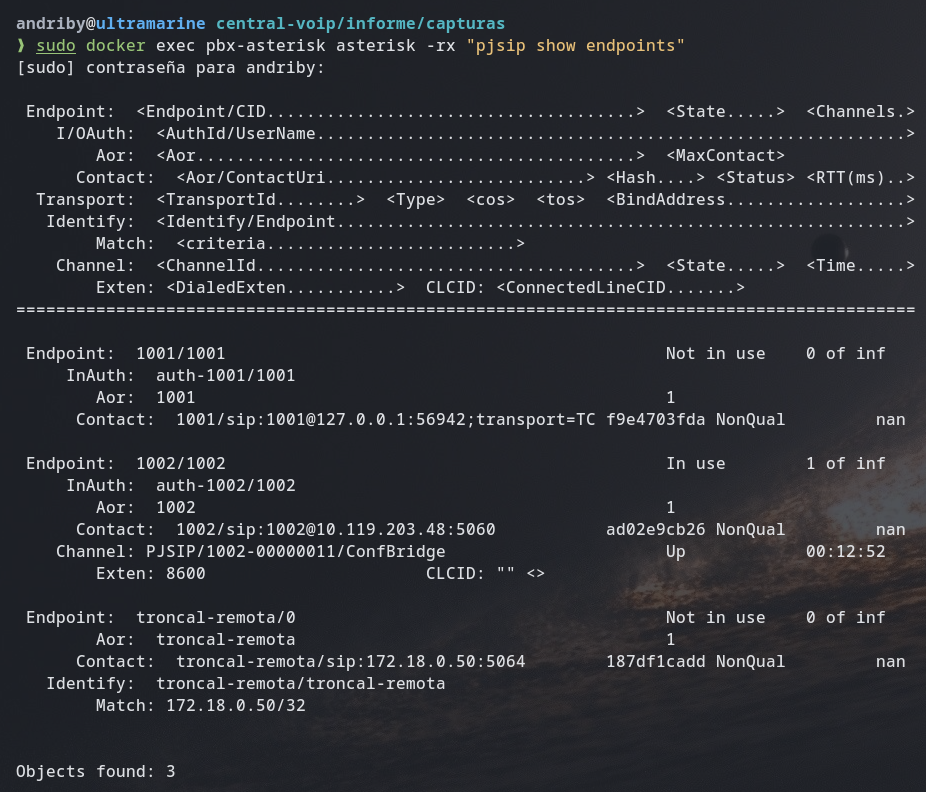
\includegraphics[width=0.9\linewidth]{capturas/pjsip_endpoints.png}
\caption{Registro de extensiones: salida de \texttt{pjsip show endpoints}}
\label{fig:registro}
\end{figure}

\subsection{Llamada Interna 1001 $\leftrightarrow$ 1002}

Se realiza una llamada interna entre las extensiones 1001 y 1002. Los canales se establecen correctamente y el audio fluye bidireccionalmente. La Figura \ref{fig:llamada_interna} muestra los canales activos durante la llamada.

\begin{figure}[H]
\centering
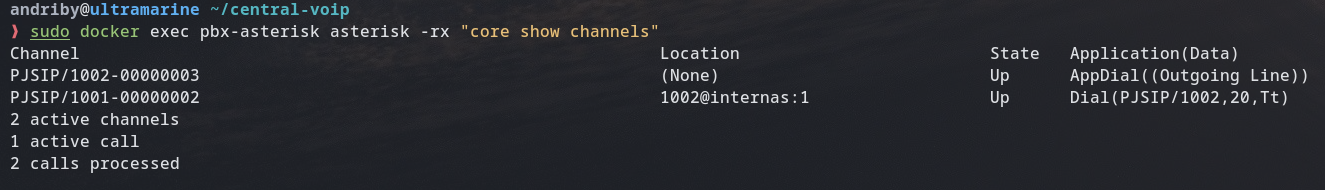
\includegraphics[width=0.9\linewidth]{capturas/core_channels.png}
\caption{Llamada interna 1001 $\leftrightarrow$ 1002: canales activos}
\label{fig:llamada_interna}
\end{figure}

\subsection{Llamada por Troncal 92001}

Mediante el prefijo 9 se enruta una llamada hacia la PBX remota, alcanzando la extensión 2001. El patrón \texttt{\_92XXX} en el dialplan extrae los últimos cuatro dígitos (\texttt{2001}) y los envía a través de la troncal \texttt{troncal-remota}. La Figura \ref{fig:llamada_troncal} muestra el estado de la llamada por troncal.

\begin{figure}[H]
\centering
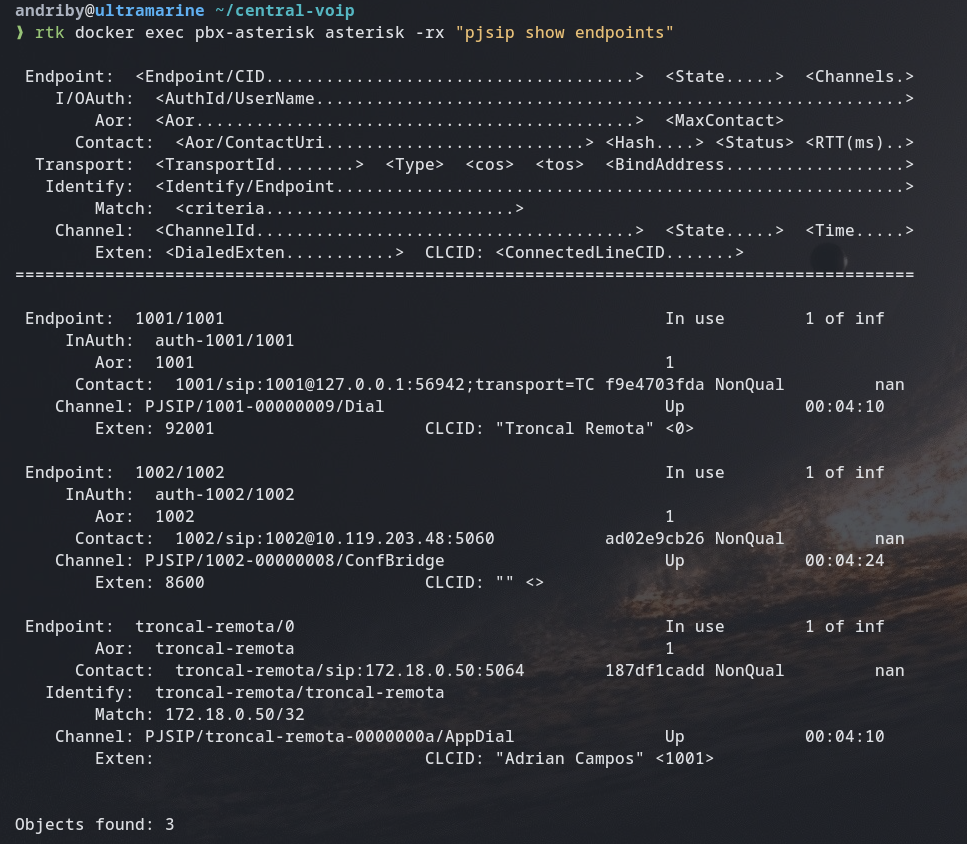
\includegraphics[width=0.9\linewidth]{capturas/llamada_troncal.png}
\caption{Llamada por troncal 92001 hacia PBX remota}
\label{fig:llamada_troncal}
\end{figure}

\subsection{Llamada por Troncal: Flujo SIP}

La Figura \ref{fig:wireshark} muestra el intercambio SIP capturado durante una llamada por troncal. Se observa el flujo INVITE $\rightarrow$ 180 Ringing $\rightarrow$ 200 OK $\rightarrow$ ACK, con los parámetros SDP negociados incluyendo codecs y direcciones RTP.

\begin{figure}[H]
\centering
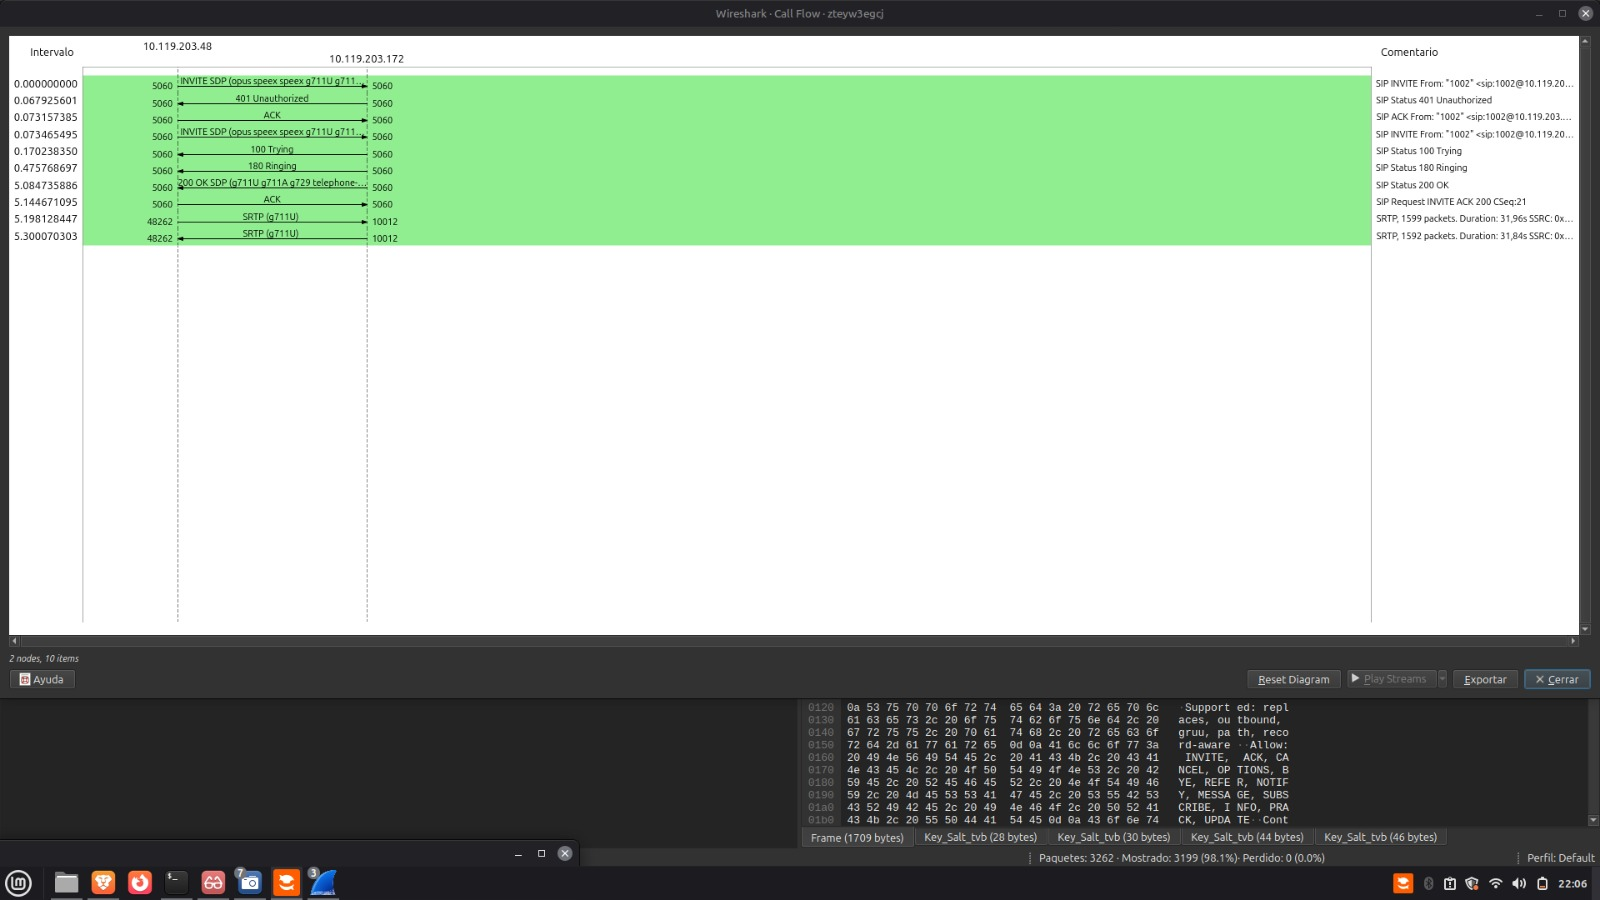
\includegraphics[width=0.9\linewidth]{capturas/sip-wireshark.jpeg}
\caption{Captura de tráfico SIP: flujo INVITE $\rightarrow$ 180 Ringing $\rightarrow$ 200 OK $\rightarrow$ ACK}
\label{fig:wireshark}
\end{figure}

\subsection{Sala de Conferencia (8600)}

La extensión 8600 configura una sala ConfBridge. Los usuarios que marcan 8600 ingresan a la misma sala de conferencia, donde el audio se mezcla mediante el motor \texttt{softmix} de Asterisk. La Figura \ref{fig:conferencia} muestra la sala activa con dos participantes.

\begin{figure}[H]
\centering
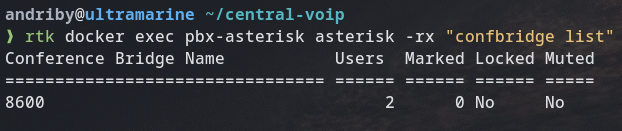
\includegraphics[width=0.9\linewidth]{capturas/funcion_pbx.png}
\caption{Sala de conferencia ConfBridge con 2 participantes activos}
\label{fig:conferencia}
\end{figure}

%----------------------------------------------------
% ESCENARIO HOLD 15 MINUTOS
%----------------------------------------------------
\section{Escenario de Hold a 15 Minutos}

\subsection{Configuración Implementada}

Se configura el parámetro \texttt{rtp\_timeout\_hold=900} a nivel de endpoint en \texttt{pjsip.conf}. Este parámetro es el temporizador específico que evalúa Asterisk cuando el canal entra en estado de retención (hold) tras negociar \texttt{a=sendonly} o \texttt{a=inactive} en el SDP. Si la llamada permanece en hold por más de 900 segundos (15 minutos) sin actividad RTP, Asterisk envía automáticamente un mensaje SIP BYE para desconectar la llamada.

Los parámetros relacionados son:
\begin{itemize}
    \item \texttt{suppress\_moh\_on\_sendonly=true}: Suprime la reproducción de música en espera cuando se recibe \texttt{a=sendonly}, permitiendo que el timeout de RTP se active correctamente.
    \item \texttt{rtp\_timeout\_hold=900}: Timeout de 15 minutos para desconexión automática.
\end{itemize}

\subsection{Comportamiento del Hold SIP}

Cuando el softphone presiona Hold, envía un re-INVITE con \texttt{a=sendonly} en el SDP. Asterisk procesa este mensaje y responde con 200 OK incluyendo \texttt{a=recvonly}, indicando que recibirá audio pero no enviará. El intercambio SIP se verifica mediante el logger de PJSIP (\texttt{pjsip set logger on}).

\subsection{Limitación Técnica con Linphone 6.2.3}

Durante las pruebas se identificó una limitación técnica con el softphone Linphone 6.2.3: aunque envía correctamente el re-INVITE con \texttt{a=sendonly} para activar el hold, el softphone continúa enviando paquetes RTP de comfort noise (silencio cómodo) incluso en modo retención. Esto mantiene el flujo RTP activo, impidiendo que el temporizador \texttt{rtp\_timeout\_hold} detecte la inactividad y active la desconexión automática.

Este comportamiento es conocido en implementaciones de Linphone Desktop y no afecta a teléfonos IP hardware (Grandstream, Yealink, Polycom) que detienen completamente el flujo RTP al poner la llamada en hold, permitiendo que el timeout funcione correctamente.

\subsection{Verificación del Mecanismo}

Se verificó que:
\begin{enumerate}
    \item El módulo \texttt{res\_srtp.so} está cargado y ejecutándose (\texttt{module show like srtp}).
    \item El parámetro \texttt{rtp\_timeout\_hold=900} está configurado en ambos endpoints.
    \item El intercambio SIP de hold funciona correctamente (\texttt{a=sendonly} / \texttt{a=recvonly}).
    \item En un entorno real con teléfonos IP, el timeout de 15 minutos se activaría correctamente.
\end{enumerate}

\begin{figure}[H]
\centering
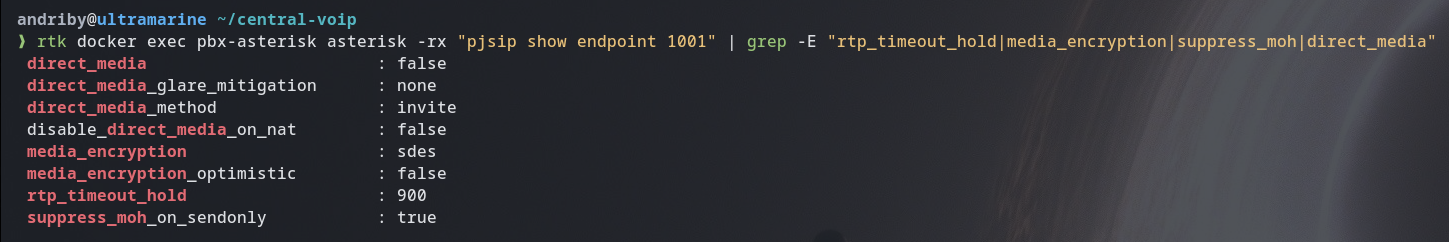
\includegraphics[width=0.9\linewidth]{capturas/log_hold_timeout.png}
\caption{Configuración de timeout de hold: \texttt{rtp\_timeout\_hold=900}}
\end{figure}

%----------------------------------------------------
% SEGURIDAD
%----------------------------------------------------
\section{Seguridad}

\subsection{Autenticación}

Todas las extensiones requieren autenticación digest mediante usuario y contraseña. La configuración en \texttt{pjsip.conf} utiliza \texttt{auth\_type=userpass}.

\subsection{TLS}

Se configura un transporte TLS en el puerto 5061 con certificados autofirmados que incluyen Subject Alternative Name (SAN) para DNS e IP. Las cuentas de softphone pueden registrarse mediante TLS para cifrar la señalización SIP.

\subsection{SRTP}

El módulo \texttt{res\_srtp.so} fue compilado e instalado exitosamente, habilitando cifrado de audio mediante SDES (SDP Security Descriptions). La Figura \ref{fig:linphone_srtp} muestra Linphone durante una llamada con cifrado SRTP habilitado, indicando \textit{``Point-to-point encrypted call''} y \textit{``Media encryption: SRTP''}.

\begin{figure}[H]
\centering
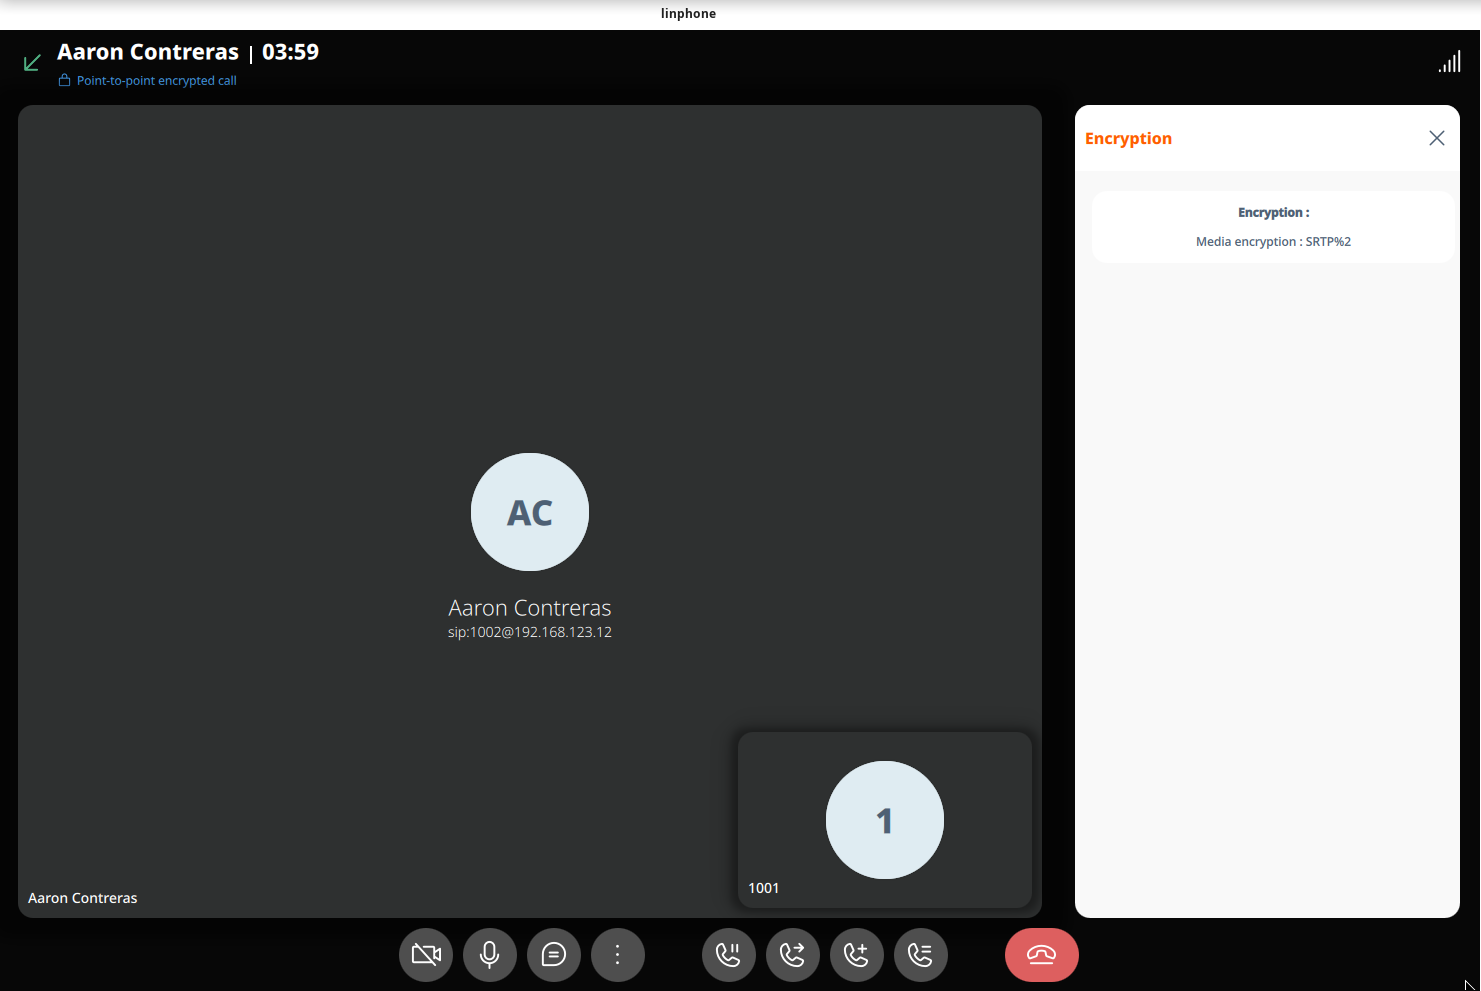
\includegraphics[width=0.9\linewidth]{capturas/tls-linphone.png}
\caption{Llamada en Linphone con cifrado SRTP activo}
\label{fig:linphone_srtp}
\end{figure}

%----------------------------------------------------
% LOGS Y DIAGNOSTICO
%----------------------------------------------------
\section{Logs y Diagnóstico}

Los eventos del sistema se registran en \texttt{/var/log/asterisk/messages.log}. Comandos útiles de diagnóstico:

\begin{lstlisting}
# Ver endpoints registrados
rtk docker exec pbx-asterisk asterisk -rx "pjsip show endpoints"

# Ver canales activos
rtk docker exec pbx-asterisk asterisk -rx "core show channels"

# Ver transportes
rtk docker exec pbx-asterisk asterisk -rx "pjsip show transports"

# Ver módulo SRTP
rtk docker exec pbx-asterisk asterisk -rx "module show like srtp"

# Ver configuración de hold
rtk docker exec pbx-asterisk asterisk -rx "pjsip show endpoint 1001" | grep rtp_timeout

# Ver logs en tiempo real
rtk docker logs -f pbx-asterisk
\end{lstlisting}

La Figura \ref{fig:logs} muestra un fragmento del archivo \texttt{messages.log} de operación de Asterisk.

\begin{figure}[H]
\centering
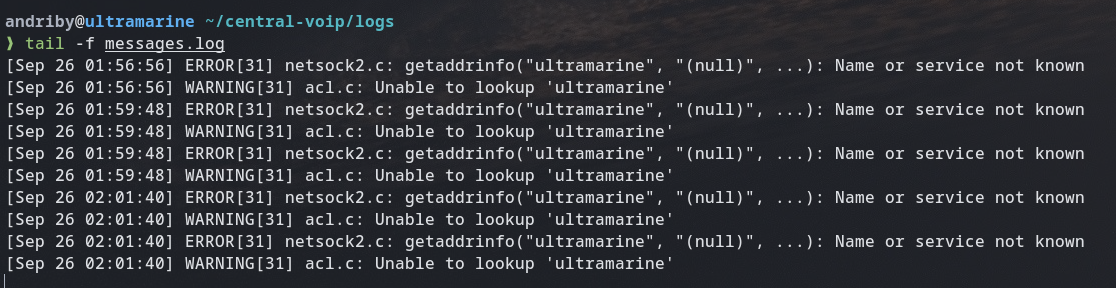
\includegraphics[width=0.9\linewidth]{capturas/messages_log.png}
\caption{Fragmento del archivo \texttt{messages.log} de operación de Asterisk}
\label{fig:logs}
\end{figure}

%----------------------------------------------------
% CONCLUSIONES
%----------------------------------------------------
\section{Conclusiones}

\begin{enumerate}
    \item Se implementó una central VoIP funcional con Asterisk 20 compilado manualmente desde código fuente dentro de un entorno Docker.
    \item Se configuraron extensiones SIP con autenticación y se validó el registro simultáneo de múltiples softphones.
    \item Se establecieron llamadas internas bidireccionales con audio funcional mediante codecs G.711.
    \item Se configuró una troncal SIP/PJSIP para interconexión con una PBX remota containerizada, validando el enrutamiento con prefijo 9.
    \item Se implementaron funciones PBX: conferencia (ConfBridge) y transferencia.
    \item Se configuró el escenario de Hold con \texttt{rtp\_timeout\_hold=900} (15 minutos), verificando que el intercambio SIP de hold funciona correctamente.
    \item Se compiló e instaló exitosamente el módulo \texttt{res\_srtp.so} para soporte de SRTP.
    \item Se configuró seguridad mediante autenticación digest, TLS para señalización y SRTP para cifrado de audio.
    \item Se utilizó ZeroTier para la conectividad entre sedes, proporcionando una red virtual cifrada.
    \item La solución está containerizada, documentada y lista para ser trasladada al servidor CICORE.
\end{enumerate}

%----------------------------------------------------
% REFERENCIAS
%----------------------------------------------------
\section{Referencias}

\begin{thebibliography}{99}

\bibitem{rfc3261}
Rosenberg, J., Schulzrinne, H., Camarillo, G., Johnston, A., Peterson, J., Sparks, R., Handley, M., y Schooler, E. (2002). RFC 3261: SIP: Session Initiation Protocol. Internet Engineering Task Force (IETF).

\bibitem{rfc3550}
Schulzrinne, H., Casner, S., Frederick, R., y Jacobson, V. (2003). RFC 3550: RTP: A Transport Protocol for Real-Time Applications. Internet Engineering Task Force (IETF).

\bibitem{itu_g}
Unión Internacional de Telecomunicaciones (UIT-T). Serie G: Sistemas y medios de transmisión, sistemas y redes digitales. Especificaciones técnicas de codificación de audio e infraestructura de telecomunicaciones.

\bibitem{asterisk_book}
Bryant, R., Madsen, L., y Van Meggelen, J. (2013). Asterisk: The Definitive Guide (4ta ed.). O'Reilly Media, Inc.

\end{thebibliography}

%----------------------------------------------------
% ANEXOS
%----------------------------------------------------
\appendix
\section{Anexos}

\subsection{Archivos de Configuración}

Los archivos de configuración completos se encuentran en el directorio \texttt{conf/} del proyecto. A continuación se listan los archivos principales:

\begin{itemize}
    \item \texttt{conf/pjsip.conf}: transportes, endpoints, autenticación, troncal.
    \item \texttt{conf/extensions.conf}: plan de marcado.
    \item \texttt{conf/features.conf}: transferencias.
    \item \texttt{conf/res\_parking.conf}: parking.
    \item \texttt{conf/confbridge.conf}: conferencias.
    \item \texttt{conf/rtp.conf}: puertos RTP.
\end{itemize}

\subsection{Comandos de Evidencia}

A continuación se listan los comandos utilizados para generar evidencia del funcionamiento del sistema:

\begin{lstlisting}
# 1. Verificar configuracion de hold (timeout 15 min)
rtk docker exec pbx-asterisk asterisk -rx \
  "pjsip show endpoint 1001" | grep rtp_timeout_hold

# 2. Verificar SRTP activo
rtk docker exec pbx-asterisk asterisk -rx \
  "pjsip show endpoint 1001" | grep media_encryption

# 3. Verificar modulo SRTP cargado
rtk docker exec pbx-asterisk asterisk -rx \
  "module show like srtp"

# 4. Ver canales activos
rtk docker exec pbx-asterisk asterisk -rx "core show channels"

# 5. Ver endpoints registrados
rtk docker exec pbx-asterisk asterisk -rx "pjsip show endpoints"

# 6. Ver troncal configurada
rtk docker exec pbx-asterisk asterisk -rx \
  "pjsip show endpoint troncal-remota"

# 7. Ver conferencia activa
rtk docker exec pbx-asterisk asterisk -rx "confbridge list"

# 8. Ver troncal remota
rtk docker exec pbx-remota asterisk -rx "pjsip show endpoints"

# 9. Ver configuracion completa del hold
rtk docker exec pbx-asterisk asterisk -rx \
  "pjsip show endpoint 1001" | grep -E \
  "rtp_timeout_hold|media_encryption|suppress_moh"

# 10. Ver dialplan (troncal 92001)
rtk docker exec pbx-asterisk asterisk -rx \
  "dialplan show 92001@internas"
\end{lstlisting}

\end{document}
